\documentclass[aps,prb,10pt,letterpaper,notitlepage]{revtex4-1}
\usepackage{amsmath}
\usepackage{subcaption}
\usepackage{graphicx}

\usepackage[colorlinks=true]{hyperref}

\begin{document}

\title{Expressions for arbitrary rotation on
\texorpdfstring{$\boldsymbol{\chi}(-2\omega;\omega,\omega)$}{X(2w)}}
\author{Sean M. Anderson}
    \email{sma@cio.mx}
    \affiliation{Centro de Investigaciones en \'Optica, A.C., Le\'on 37150,
    Mexico}
\author{Yujin Cho}
    \affiliation{Department of Physics, University of Texas at Austin, Austin,
    Texas 78712, USA}
\author{Bernardo S. Mendoza}
    \affiliation{Centro de Investigaciones en \'Optica, A.C., Le\'on 37150,
    Mexico}
\date{\today}

\begin{abstract}
We develop the explicit expressions for rotating the nonlinear susceptibility
tensor $\boldsymbol{\chi}(-2\omega;\omega,\omega)$ through any arbitrary angle.
Each component in the rotated frame of reference is a combination of different
components from the non-rotated system; setting the angle of rotation to $\pi/2$
is equivalent to no rotation whatsoever.
\end{abstract}

\maketitle

To take the components of $\boldsymbol{\chi}(-2\omega;\omega,\omega)$ from the
crystallographic frame to the lab frame, we can simply apply a standard
rotational matrix,
\begin{equation*}
R =
\begin{pmatrix}
R_{Xx} & R_{Xy} & R_{Xz} \\
R_{Yx} & R_{Yy} & R_{Yz} \\
R_{Zx} & R_{Zy} & R_{Zz} \\
\end{pmatrix}
=
\begin{pmatrix}
\sin\Phi & -\cos\Phi & 0 \\
\cos\Phi &  \sin\Phi & 0 \\
    0    &      0    & 1
\end{pmatrix},
\end{equation*}
such that
\begin{equation*}
\chi^{IJK} = \sum_{ijk}R_{Ii}R_{Jj}R_{Kk}\chi^{ijk},
\end{equation*}
where $I$, $J$, and $K$ ($i$, $j$, $k$) cycle through $X$, $Y$, or $Z$ ($x$,
$y$, $z$). Fig. \ref{fig:axes} depicts this rotation over any arbitrary
combination of angles $\Theta$ and $\Phi$; however, in this work we will only
consider a rotation in the $xy$-plane along $\Phi$.

\begin{figure}[b]
\centering
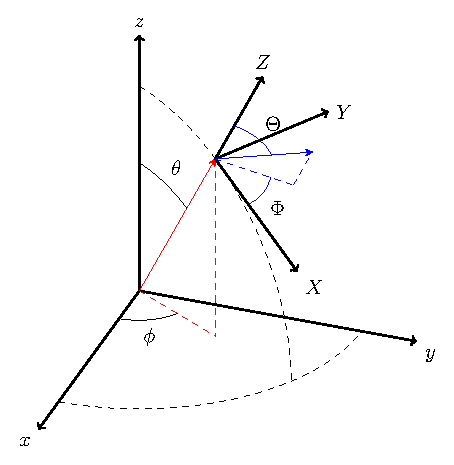
\includegraphics[width=0.4\linewidth]{axes}
\caption{The translation from the non-rotates $xyz$ coordinates to the rotated
$XYZ$ system. In this work, we will only consider an in-plane rotation of
$\Phi$.}
\label{fig:axes}
\end{figure}

Thus, our $\chi^{IJK}$ components in terms of the original $ijk$ coordinate
system are
\begin{equation}\label{eq:xcomps}
\begin{split}
\chi^{XXX} 
&=  \sin^{3}\Phi          \chi^{xxx}
 +  \sin\Phi \cos^{2}\Phi \chi^{xyy}
 - 2\sin^{2}\Phi \cos\Phi \chi^{xxy}\\
&-  \sin^{2}\Phi \cos\Phi \chi^{yxx}
 -  \cos^{3}\Phi          \chi^{yyy}
 + 2\sin\Phi \cos^{2}\Phi \chi^{yxy},\\[10pt]
%%%%%%%%%%%%%%%%%%%%%%%%%%%%%%%%%%%%%%%%%%%%%%%%%%
\chi^{XYY} 
&=  \sin\Phi \cos^{2}\Phi \chi^{xxx}
 +  \sin^{3}\Phi          \chi^{xyy}
 + 2\sin^{2}\Phi \cos\Phi \chi^{xxy}\\
&-  \cos^{3}\Phi          \chi^{yxx}
 -  \sin^{2}\Phi \cos\Phi \chi^{yyy}
 - 2\sin\Phi \cos^{2}\Phi \chi^{yxy},\\[10pt]
%%%%%%%%%%%%%%%%%%%%%%%%%%%%%%%%%%%%%%%%%%%%%%%%%%
\chi^{XZZ} 
&= \sin\Phi \chi^{xzz}
 - \cos\Phi \chi^{yzz},\\[10pt]
%%%%%%%%%%%%%%%%%%%%%%%%%%%%%%%%%%%%%%%%%%%%%%%%%%
\chi^{XYZ} = \chi^{XZY}
&=
   \sin^{2}\Phi      \chi^{xyz}
 + \sin\Phi \cos\Phi \chi^{xxz}
 - \sin\Phi \cos\Phi \chi^{yyz}
 - \cos^{2}\Phi      \chi^{yxz},\\[10pt]
%%%%%%%%%%%%%%%%%%%%%%%%%%%%%%%%%%%%%%%%%%%%%%%%%%
\chi^{XXZ} = \chi^{XZX}
&=
 - \sin\Phi \cos\Phi \chi^{xyz}
 + \sin^{2}\Phi      \chi^{xxz}
 + \cos^{2}\Phi      \chi^{yyz}
 - \sin\Phi \cos\Phi \chi^{yxz},\\[10pt]
%%%%%%%%%%%%%%%%%%%%%%%%%%%%%%%%%%%%%%%%%%%%%%%%%%
\chi^{XXY} = \chi^{XYX} 
&= 
   \sin^{2}\Phi \cos\Phi \chi^{xxx}
 - \sin^{2}\Phi \cos\Phi \chi^{xyy}
 + (\sin^{3}\Phi - \sin\Phi \cos^{2}\Phi) \chi^{xxy}\\
&- \sin\Phi \cos^{2}\Phi \chi^{yxx}
 + \sin\Phi \cos^{2}\Phi \chi^{yyy}
 + (\cos^{3}\Phi - \sin^{2}\Phi \cos\Phi) \chi^{yxy},
\end{split}
\end{equation}
for the $\chi^{XJK}$ components,
\begin{equation*}
\begin{split}
\chi^{YXX}
&=  \sin^{2}\Phi \cos\Phi \chi^{xxx}
 +  \cos^{3}\Phi          \chi^{xyy}
 - 2\sin\Phi \cos^{2}\Phi \chi^{xxy}\\
&+  \sin^{3}\Phi          \chi^{yxx}
 +  \sin\Phi \cos^{2}\Phi \chi^{yyy}
 - 2\sin^{2}\Phi \cos\Phi \chi^{yxy},\\[10pt]
%%%%%%%%%%%%%%%%%%%%%%%%%%%%%%%%%%%%%%%%%%%%%%%%%%
\chi^{YYY}
&=  \cos^{3}\Phi          \chi^{xxx}
 +  \sin^{2}\Phi \cos\Phi \chi^{xyy}
 + 2\sin\Phi \cos^{2}\Phi \chi^{xxy}\\
&+  \sin\Phi \cos^{2}\Phi \chi^{yxx}
 +  \sin^{3}\Phi          \chi^{yyy}
 + 2\sin^{2}\Phi \cos\Phi \chi^{yxy},\\[10pt]
%%%%%%%%%%%%%%%%%%%%%%%%%%%%%%%%%%%%%%%%%%%%%%%%%%
\chi^{YZZ}
&= \cos\Phi \chi^{xzz} + \sin\Phi \chi^{yzz},\\[10pt]
%%%%%%%%%%%%%%%%%%%%%%%%%%%%%%%%%%%%%%%%%%%%%%%%%%
\chi^{YYZ} = \chi^{YZY}
&= \sin\Phi \cos\Phi \chi^{xyz}
 + \cos^{2}\Phi      \chi^{xxz}
 + \sin^{2}\Phi      \chi^{yyz}
 + \sin\Phi \cos\Phi \chi^{yxz},\\[10pt]
%%%%%%%%%%%%%%%%%%%%%%%%%%%%%%%%%%%%%%%%%%%%%%%%%%
\chi^{YXZ} = \chi^{YZX}
&=
- \cos^{2}\Phi      \chi^{xyz}
+ \sin\Phi \cos\Phi \chi^{xxz}
- \sin\Phi \cos\Phi \chi^{yyz}
+ \sin^{2}\Phi      \chi^{yxz},\\[10pt]
%%%%%%%%%%%%%%%%%%%%%%%%%%%%%%%%%%%%%%%%%%%%%%%%%%
\chi^{YXY} = \chi^{YYX}
&= \sin\Phi \cos^{2}\Phi \chi^{xxx}
 - \sin\Phi \cos^{2}\Phi \chi^{xyy}
 + (\sin^{2}\Phi \cos\Phi - \cos^{3}\Phi) \chi^{xxy}\\
&+ \sin^{2}\Phi \cos\Phi \chi^{yxx}
 - \sin^{2}\Phi \cos\Phi \chi^{yyy}
 + (\sin^{3}\Phi - \sin\Phi \cos^{2}\Phi) \chi^{yxy},\\[10pt]
\end{split}
\end{equation*}
for the $\chi^{YJK}$ components, and lastly
\begin{equation*}
\begin{split}
\chi^{ZXX}
&=  \sin^{2}\Phi      \chi^{zxx}
 +  \cos\Phi \cos\Phi \chi^{zyy}
 - 2\sin\Phi \cos\Phi \chi^{zxy},\\[10pt]
%%%%%%%%%%%%%%%%%%%%%%%%%%%%%%%%%%%%%%%%%%%%%%%%%%
\chi^{ZYY}
&=  \cos^{2}\Phi      \chi^{zxx}
 +  \sin^{2}\Phi      \chi^{zyy}
 + 2\sin\Phi \cos\Phi \chi^{zxy},\\[10pt]
%%%%%%%%%%%%%%%%%%%%%%%%%%%%%%%%%%%%%%%%%%%%%%%%%%
\chi^{ZZZ} &=  \chi^{zzz},\\[10pt]
%%%%%%%%%%%%%%%%%%%%%%%%%%%%%%%%%%%%%%%%%%%%%%%%%%
\chi^{ZYZ} = \chi^{ZZY}
&= \sin\Phi \chi^{zyz}
 + \cos\Phi \chi^{zxz},\\[10pt]
%%%%%%%%%%%%%%%%%%%%%%%%%%%%%%%%%%%%%%%%%%%%%%%%%%
\chi^{ZXZ} = \chi^{ZZX}
&= 
- \cos\Phi \chi^{zyz}
+ \sin\Phi \chi^{zxz},\\[10pt]
%%%%%%%%%%%%%%%%%%%%%%%%%%%%%%%%%%%%%%%%%%%%%%%%%%
\chi^{ZXY} = \chi^{ZYX}
&= \sin\Phi \cos\Phi \chi^{zxx}
 - \sin\Phi \cos\Phi \chi^{zyy}
 - \cos2\Phi         \chi^{zxy},
\end{split}
\end{equation*}
for the $\chi^{ZJK}$ components. Fortunately, the intrinsic permutation symmetry
of SHG is also present in the new coordinate system, such that $\chi^{IJK} =
\chi^{IKJ}$; therefore, there are only 18 unique components in either system.
Setting $\Phi = \pi/2$ signifies that there is no rotation, and thus $\chi^{IJK}
= \chi^{ijk}$.

It should also be clear that the crystal symmetries do \textbf{not} follow into
the rotated system. For instance, the $C_{3v}$ symmetry satisfies the following,
\begin{equation*}
\begin{split}
\chi^{xxx} &= -\chi^{xyy} = - \chi^{yxy},\\
\chi^{yxx} &= \chi^{yyy} = 0.
\end{split}
\end{equation*}
In the rotated system, the top relationship holds true such that $\chi^{XXX} =
-\chi^{XYY} = - \chi^{YXY}$. However, we also obtain that
\begin{equation*}
\chi^{YYY} = \cos3\Phi \chi^{xxx},
\end{equation*}
which is most definitely not zero. Fortunately, we can simply apply the crystal
symmetry to the non-rotated system before transforming to the rotated system.

As an example case, we present $\chi^{XXX}$ for three values of $\Phi$ for a
system with $C_{3v}$ symmetry in Fig. \ref{fig:rotxxx}. The nonzero components
in the original coordinates are presented in Fig. \ref{fig:comps}, multiplied by
the appropriate prefactors from Eq. \eqref{eq:xcomps}. We can see how we recover
the component in the original coordinates when $\Phi = \pi/2$.

\begin{figure}[t]
\centering
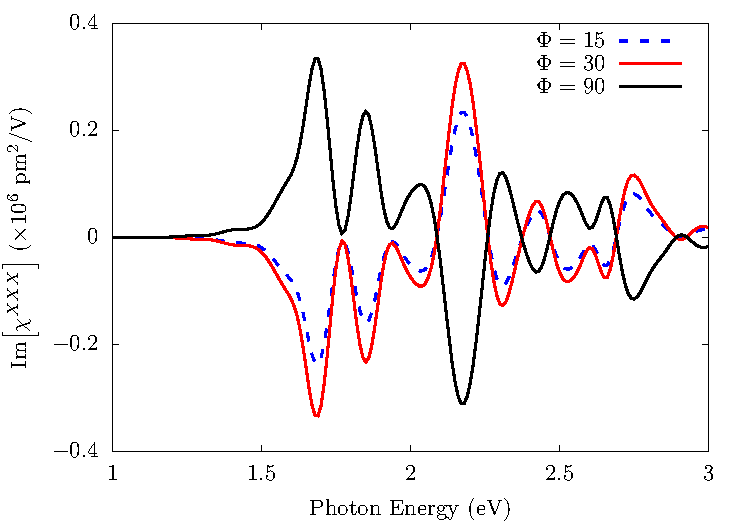
\includegraphics[width=0.4\linewidth]{rot/rotxxx.pdf}
\caption{$\chi^{XXX}$ for three values of $\Phi$ calculated for a system with
$C_{3v}$ symmetry.}
\label{fig:rotxxx}
\end{figure}

\begin{figure}[b]
    \centering
    \begin{subfigure}[b]{0.25\textwidth}
        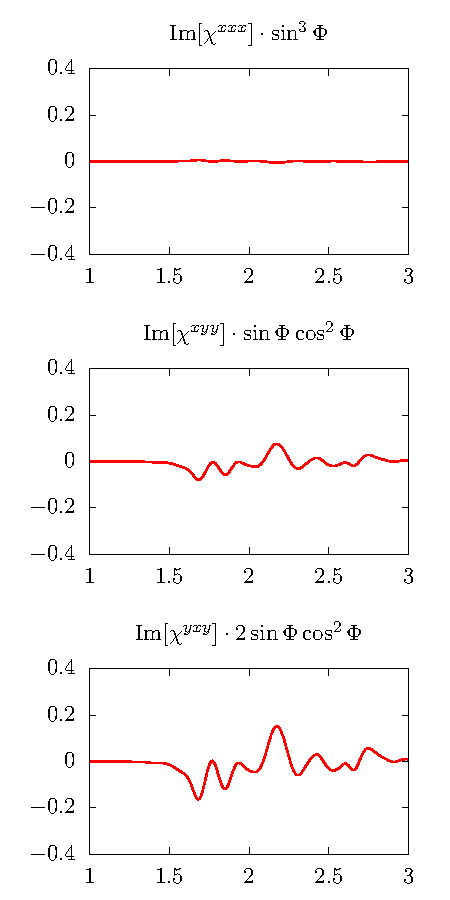
\includegraphics[width=0.8\textwidth]{rot/comps15.pdf}
        \caption{$\Phi = \pi/12$.}
    \end{subfigure}
    ~ 
    \begin{subfigure}[b]{0.25\textwidth}
        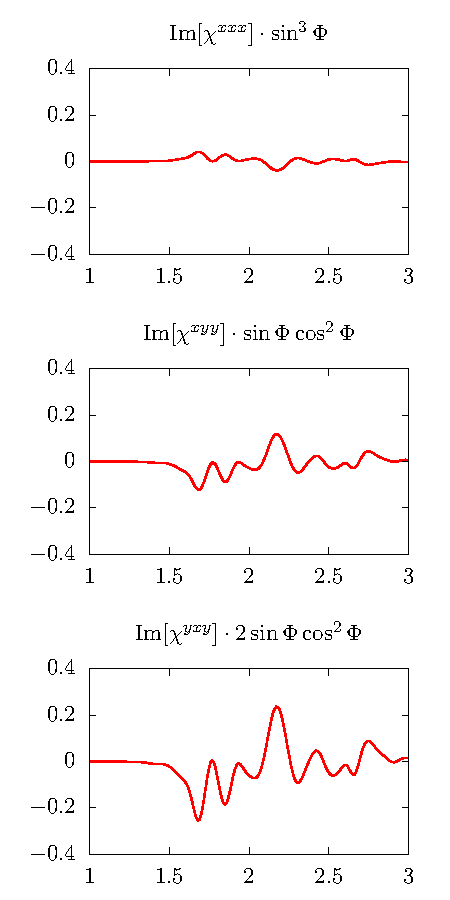
\includegraphics[width=0.8\textwidth]{rot/comps30.pdf}
        \caption{$\Phi = \pi/6$.}
    \end{subfigure}
    ~ 
    \begin{subfigure}[b]{0.25\textwidth}
        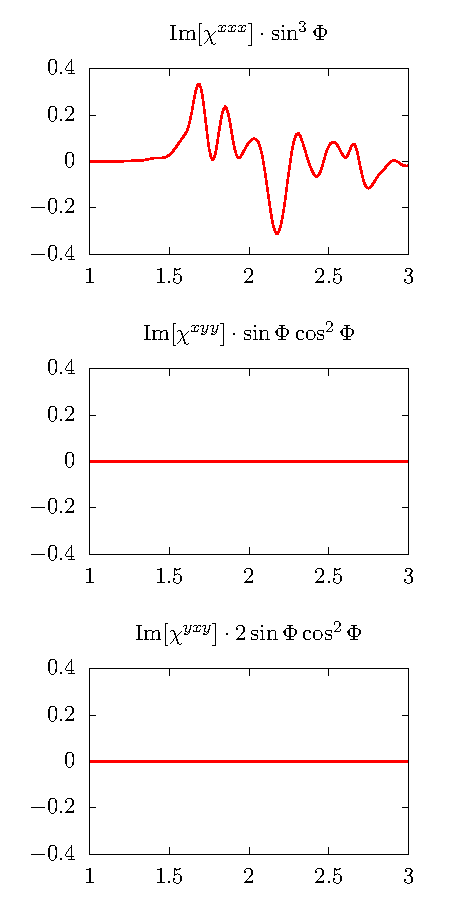
\includegraphics[width=0.8\textwidth]{rot/comps90.pdf}
        \caption{$\Phi = \pi/2$.}
    \end{subfigure}
    \caption{Nonzero components of $\chi^{ijk}$ multiplied by the appropriate
    prefactors, for three different values of $\Phi$.}
    \label{fig:comps}
\end{figure}


\end{document}
